\section{Commissioning}

To do the initial commissioning, some repeatable test setup is required.

When the boards arrive from the factory, all \ac{smd} components are already assembled. Any missing components are then assembled by hand using a soldering iron. This includes at least one pin socket or header for most boards. Other boards may also require additional \ac{tht} components such as diodes. When all components are installed on the board, testing can begin. Since the manufacturer of the boards does flyprobe tests on all produced boards after \ac{smd} assembly, only one board per type is tested for functionality. To do so, a temporary testing harness is attached, connecting the device to a testing microcontroller. In this case, the microcontroller of choice is the ATMEGA 2560, mounted on the popular breakout board "Arduino MEGA". This board was chosen because it was already available at hand and exposes more than 40 digital IO pins, as well as the previous experience of the author with the board. It is programmable via USB and due to the widely used "Arduino" framework, commissioning and deployment of testing code was vastly sped up. The board can be seen in \autoref{fig:arduino_mega}.

\begin{figure}[h!]
    \centering
    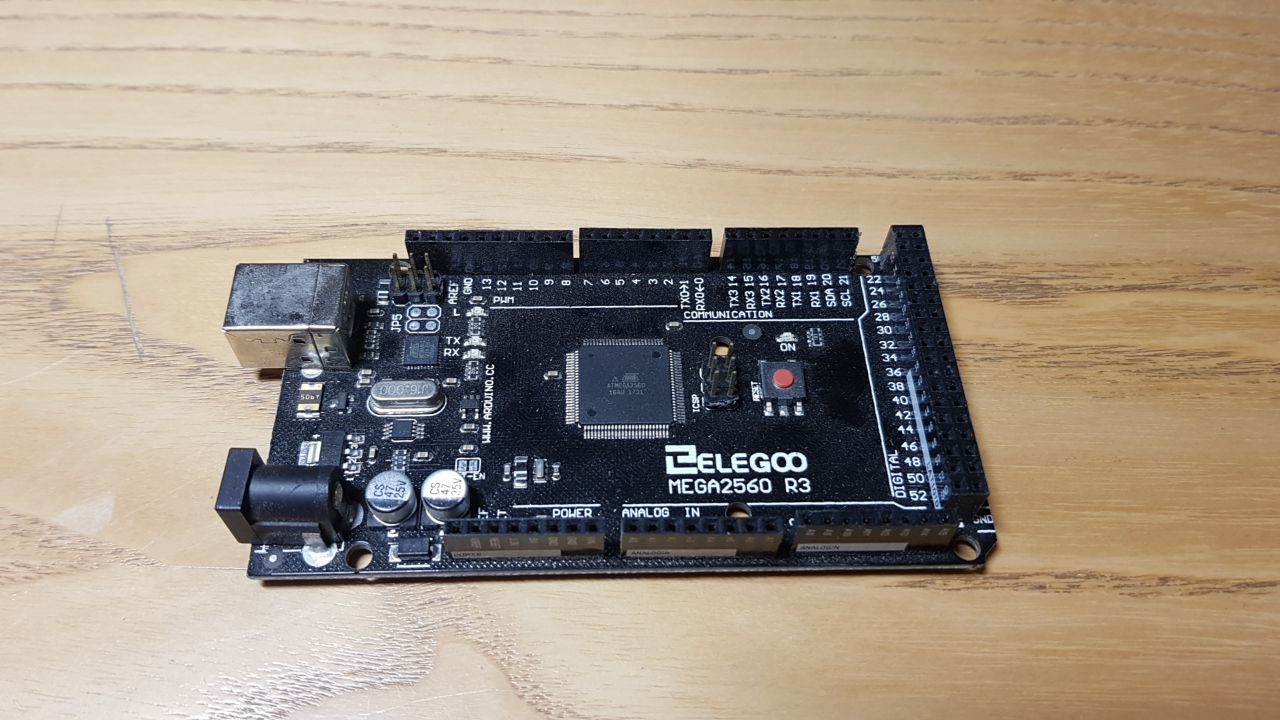
\includegraphics[width=\textwidth]{images/arduino_mega.jpg}
    \caption{Elegoo MEGA2560 development board (compatible with the Arduino MEGA)}
    \label{fig:arduino_mega}
\end{figure}

The testing harness consists of individual wires and sections of ribbon cables with 2.54mm Dupont connectors. All ground pins of the \ac{dut} are connected to the common ground of both the main power supply, as well as the ATMEGA. The anode terminal of the power supply is then connected to all supply pins of the \ac{dut}. All other pins are signal pins, which are connected to the digital IO pins of the ATMEGA. The ATMEGA is additionally connected to a host computer via USB in order to compile and upload test software, as well as to read back the results. \autoref{fig:register_in_testing_harness} shows a register \ac{pcb} in its testing harness, which was the first board to be tested for the project.

\begin{figure}[h!]
    \centering
    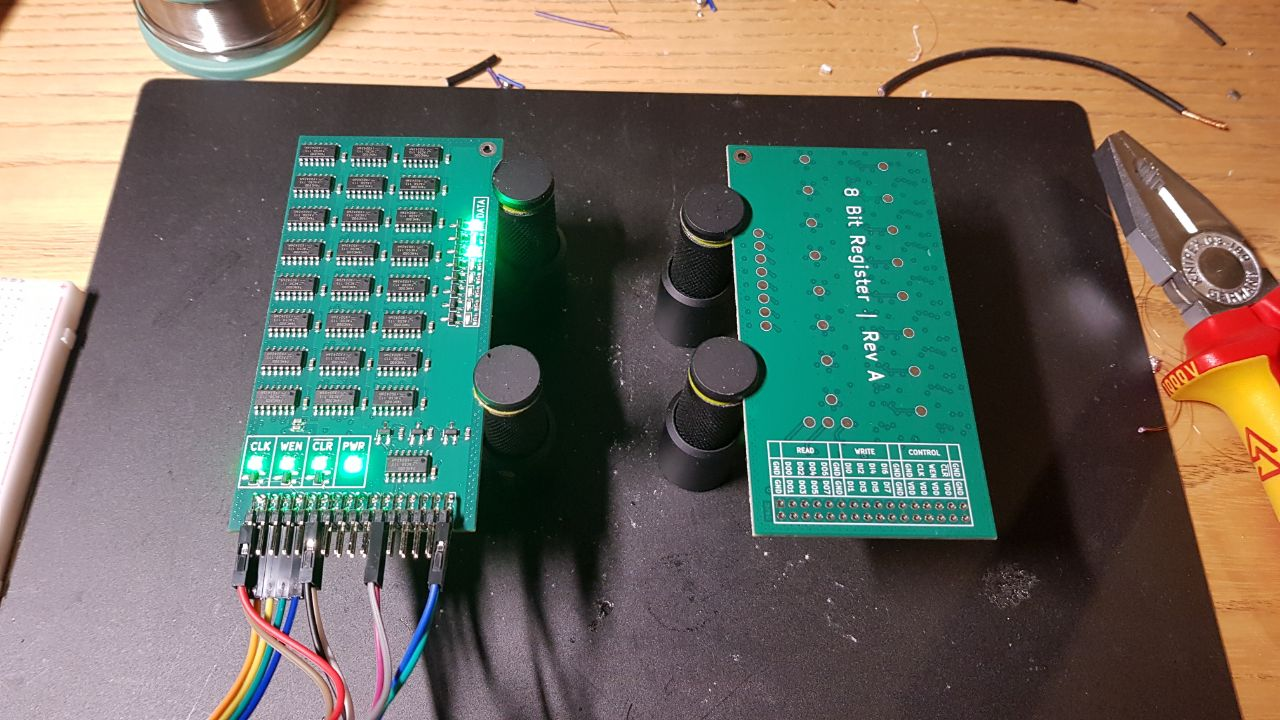
\includegraphics[width=\textwidth]{images/register_in_test_jig.jpg} % Replace with your image file
    \caption{Register PCB in testing harness (Only ground and supply pins are connected)}
    \label{fig:register_in_testing_harness}
\end{figure}

The test software executes the same predefined tests as the simulation done for the logic design. It sets the state of all inputs to the \ac{dut}, waits a specified amount of time to allow the signal levels on the \ac{pcb} to propagate and settle, before reading back the relevant output signals. In addition to these automatic tests, the integrated \acp{led} give a visual indication of the behavior of the \ac{dut}. The first batch of \acp{pcb} that was received from the manufacturer contained only the register and adder-subtractor boards. Both of these boards worked to specification and require no further modification.
